\SourceLeaf{394}%
\begin{equation}\tag*{[4]}
\left\{\begin{aligned}
\frac{dx}{du}&=s\xi\\
\frac{dy}{du}&=s\eta\\
\frac{dz}{du}&=s\zeta;
\end{aligned}\right.
\end{equation}
[dabei wird $s$ bestimmt durch die Formel:
\begin{equation}\tag*{[5]}
ss=P\left(\frac{dt}{du}\right)^2+2Q\frac{dt}{du}\frac{d\theta}{du}+R\left(\frac{d\theta}{du}\right)^2.
\end{equation}
Zweitens ist:]
\begin{equation}\tag*{[6]}
\left\{\begin{aligned}
\frac{d\xi}{du}&=\tau\xi'\\
\frac{d\eta}{du}&=\tau\eta'\\
\frac{d\zeta}{du}&=\tau\zeta';
\end{aligned}\right.
\end{equation}
[dabei wird $\tau$ bestimmt durch die Formel:
\begin{equation}\tag*{[7]}
\tau\tau=\left(\frac{d\xi}{du}\right)^2+\left(\frac{d\eta}{du}\right)^2+\left(\frac{d\zeta}{du}\right)^2.
\end{equation}
Drittens hat man:]
\begin{equation}\tag*{[8]}
\left\{\begin{aligned}
\eta\zeta'-\zeta\eta'&=\xi''\\
\zeta\xi'-\xi\zeta'&=\eta''\\
\xi\eta'-\eta\xi'&=\zeta''.
\end{aligned}\right.
\end{equation}
\par Dann ist:
\begin{equation}\tag*{[9]}
\left\{\begin{aligned}
X\xi+Y\eta+Z\zeta&=0\\
X\xi'+Y\eta'+Z\zeta'&=-\cos\psi\\
X\xi''+Y\eta''+Z\zeta''&=+\sin\psi.
\end{aligned}\right.
\end{equation}

[Bei diesen Bezeichnungen ist]
\begin{center}
\begin{tabular}{ll}
$s\,du$&Element der Curve\\[3pt]
$\tau\,du$&Element der absoluten Krümmung\\[3pt]
$\frac{\tau}{s}$&Mass der absoluten Krümmung\\[3pt]
$\frac{\tau}{s}\cos\psi$&Mass der Normalkrümmung (nach $P$ convex)\\[3pt]
$\frac{\tau}{s}\sin\psi$&Mass der Seitenkrümmung.
\end{tabular}
\par\medskip
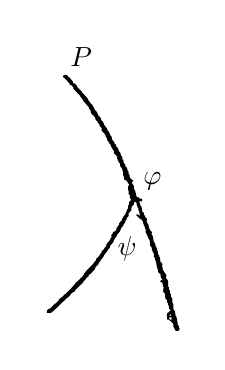
\begin{tikzpicture}[x=.00225in,y=-.00225in]
\path[use as bounding box] (0,0) rectangle (378,700);
\path[fill=black,even odd rule] (81,106) -- (79,108) -- (79,110) -- (88,118) -- (88,119) -- (93,124) -- (94,127) -- (97,128) -- (102,133) -- (102,136) -- (117,152) -- (117,153) -- (119,155) -- (119,157) -- (120,157) -- (122,159) -- (124,163) -- (136,177) -- (137,181) -- (140,184) -- (141,190) -- (151,201) -- (151,204) -- (152,206) -- (156,210) -- (156,211) -- (160,216) -- (161,220) -- (165,224) -- (165,230) -- (172,237) -- (172,239) -- (174,240) -- (174,243) -- (177,247) -- (177,250) -- (182,257) -- (182,259) -- (183,259) -- (185,261) -- (186,265) -- (192,275) -- (192,280) -- (194,282) -- (195,282) -- (200,288) -- (199,292) -- (201,294) -- (201,297) -- (203,298) -- (203,300) -- (206,303) -- (206,308) -- (211,315) -- (211,319) -- (213,321) -- (213,329) -- (214,330) -- (214,333) -- (215,334) -- (215,338) -- (217,340) -- (219,340) -- (223,344) -- (223,346) -- (226,349) -- (226,351) -- (224,354) -- (224,362) -- (225,363) -- (225,371) -- (228,374) -- (228,380) -- (230,382) -- (230,385) -- (226,389) -- (226,394) -- (224,397) -- (224,403) -- (222,405) -- (221,405) -- (221,408) -- (218,415) -- (213,422) -- (213,424) -- (211,425) -- (210,429) -- (204,436) -- (204,439) -- (201,442) -- (200,445) -- (198,447) -- (198,451) -- (195,454) -- (191,455) -- (190,458) -- (186,463) -- (187,464) -- (187,467) -- (185,469) -- (184,473) -- (176,482) -- (175,487) -- (172,490) -- (170,494) -- (165,499) -- (165,501) -- (163,503) -- (162,503) -- (162,505) -- (160,507) -- (160,508) -- (153,515) -- (152,519) -- (149,522) -- (148,522) -- (148,524) -- (145,527) -- (145,528) -- (129,544) -- (129,545) -- (126,548) -- (126,550) -- (124,552) -- (123,552) -- (122,555) -- (120,557) -- (118,557) -- (117,560) -- (106,570) -- (106,571) -- (100,577) -- (100,578) -- (84,594) -- (83,594) -- (76,601) -- (75,601) -- (71,605) -- (70,605) -- (70,607) -- (62,615) -- (60,615) -- (60,616) -- (56,620) -- (55,620) -- (55,621) -- (51,625) -- (50,625) -- (49,627) -- (47,627) -- (43,630) -- (43,635) -- (44,636) -- (52,636) -- (55,633) -- (56,633) -- (88,602) -- (90,602) -- (91,600) -- (94,597) -- (95,597) -- (95,595) -- (99,591) -- (105,588) -- (105,586) -- (108,583) -- (109,583) -- (109,582) -- (113,578) -- (114,578) -- (115,576) -- (118,573) -- (119,573) -- (123,568) -- (124,568) -- (124,566) -- (130,560) -- (130,559) -- (136,554) -- (136,552) -- (139,549) -- (140,549) -- (150,538) -- (151,534) -- (158,527) -- (158,525) -- (160,523) -- (160,522) -- (162,521) -- (162,519) -- (168,512) -- (168,511) -- (170,509) -- (170,507) -- (173,505) -- (173,503) -- (177,499) -- (179,495) -- (182,492) -- (184,488) -- (184,486) -- (191,478) -- (192,474) -- (194,472) -- (194,470) -- (198,466) -- (199,462) -- (205,455) -- (209,446) -- (214,440) -- (214,438) -- (216,436) -- (218,432) -- (218,430) -- (220,429) -- (221,424) -- (225,420) -- (225,414) -- (227,412) -- (227,411) -- (231,408) -- (231,402) -- (232,401) -- (232,399) -- (236,395) -- (237,393) -- (237,390) -- (239,388) -- (240,388) -- (243,391) -- (243,395) -- (244,396) -- (245,401) -- (247,403) -- (247,407) -- (249,410) -- (249,414) -- (250,415) -- (250,418) -- (249,419) -- (246,416) -- (243,416) -- (242,418) -- (251,427) -- (253,427) -- (257,432) -- (258,438) -- (259,439) -- (259,442) -- (261,443) -- (261,446) -- (264,452) -- (263,454) -- (264,459) -- (266,461) -- (267,465) -- (269,468) -- (269,470) -- (272,474) -- (273,486) -- (277,491) -- (277,495) -- (278,496) -- (279,501) -- (281,502) -- (281,504) -- (282,505) -- (281,510) -- (284,514) -- (284,518) -- (286,520) -- (286,523) -- (287,524) -- (287,529) -- (288,530) -- (288,534) -- (289,535) -- (289,538) -- (291,540) -- (291,545) -- (296,550) -- (297,558) -- (300,560) -- (300,561) -- (297,564) -- (296,564) -- (296,567) -- (298,567) -- (301,570) -- (301,573) -- (302,574) -- (302,577) -- (303,578) -- (302,588) -- (306,593) -- (307,604) -- (311,608) -- (311,612) -- (313,615) -- (313,618) -- (315,620) -- (315,626) -- (318,629) -- (318,631) -- (311,637) -- (311,639) -- (310,640) -- (310,642) -- (311,643) -- (311,650) -- (312,651) -- (315,651) -- (318,654) -- (319,654) -- (324,660) -- (325,662) -- (325,667) -- (330,676) -- (335,676) -- (338,674) -- (339,671) -- (337,669) -- (337,665) -- (334,662) -- (334,656) -- (333,655) -- (333,649) -- (332,648) -- (332,645) -- (330,643) -- (328,632) -- (325,628) -- (325,618) -- (323,614) -- (322,603) -- (319,599) -- (319,594) -- (317,591) -- (317,586) -- (315,584) -- (315,579) -- (313,577) -- (313,564) -- (308,558) -- (308,556) -- (309,555) -- (309,551) -- (303,543) -- (303,541) -- (301,540) -- (301,534) -- (299,532) -- (300,530) -- (300,526) -- (296,522) -- (296,519) -- (295,518) -- (295,513) -- (293,510) -- (293,507) -- (291,506) -- (290,499) -- (288,495) -- (288,491) -- (286,489) -- (285,487) -- (285,484) -- (283,481) -- (283,479) -- (281,477) -- (281,474) -- (280,473) -- (280,470) -- (279,469) -- (279,464) -- (277,463) -- (277,461) -- (276,460) -- (277,456) -- (272,450) -- (271,446) -- (270,445) -- (269,438) -- (267,436) -- (265,432) -- (266,426) -- (262,422) -- (261,419) -- (259,417) -- (259,413) -- (255,409) -- (254,399) -- (251,396) -- (250,391) -- (248,389) -- (251,386) -- (252,386) -- (253,388) -- (255,386) -- (255,382) -- (253,381) -- (250,381) -- (247,378) -- (244,378) -- (242,375) -- (242,370) -- (240,367) -- (240,364) -- (238,362) -- (238,359) -- (237,358) -- (237,353) -- (233,348) -- (233,344) -- (235,342) -- (235,341) -- (228,335) -- (228,333) -- (227,332) -- (227,328) -- (225,326) -- (225,321) -- (223,319) -- (222,315) -- (220,311) -- (218,309) -- (218,306) -- (214,301) -- (213,295) -- (211,293) -- (211,289) -- (209,287) -- (209,285) -- (207,283) -- (207,280) -- (204,276) -- (202,272) -- (202,270) -- (197,264) -- (197,261) -- (194,259) -- (193,255) -- (188,249) -- (187,243) -- (185,241) -- (182,235) -- (182,233) -- (178,229) -- (177,225) -- (170,216) -- (170,214) -- (167,209) -- (164,206) -- (164,204) -- (162,200) -- (157,195) -- (157,193) -- (155,191) -- (155,189) -- (151,185) -- (148,180) -- (148,178) -- (146,177) -- (146,175) -- (136,163) -- (133,157) -- (121,144) -- (121,143) -- (110,132) -- (110,130) -- (105,125) -- (105,124) -- (102,124) -- (101,123) -- (101,120) -- (97,116) -- (97,115) -- (86,105) -- cycle (317,645) -- (319,645) -- (321,647) -- (321,650) -- (319,652) -- (315,648) -- (315,647) -- cycle (316,640) -- (318,639) -- (320,641) -- (320,642) -- (318,643) -- (316,641) -- cycle;
\node[inner sep=0pt,font=\normalsize] at (119,66) {$P$};
\node[inner sep=0pt,font=\normalsize] at (278,342) {$\varphi$};
\node[inner sep=0pt,font=\normalsize] at (222,493) {$\psi$};
\end{tikzpicture}

\end{center}
